\documentclass[11pt]{article}
\usepackage[T1]{fontenc}
\usepackage{lmodern}
\usepackage[margin=1in]{geometry}
\usepackage{amsmath,amssymb,amsthm,mathtools}
\usepackage{microtype,booktabs,array,enumitem}
\usepackage{placeins,needspace}
\usepackage{tikz}
\usetikzlibrary{arrows.meta,calc,positioning}
\usepackage[colorlinks=true,linkcolor=black,citecolor=black,urlcolor=black]{hyperref}
\usepackage{bookmark}
\hypersetup{pdftitle={A typical-start upper bound for low-temperature SK Glauber dynamics},pdfauthor={OpenAI}}
\setlength{\emergencystretch}{3em}
\setlist{itemsep=.3em,topsep=.5em}
\setcounter{tocdepth}{1}
\allowdisplaybreaks
\newtheorem{theorem}{Theorem}
\newtheorem{lemma}[theorem]{Lemma}
\newtheorem{proposition}[theorem]{Proposition}
\newtheorem{corollary}[theorem]{Corollary}
\title{A typical-start upper bound for low-temperature\\SK Glauber dynamics}
\author{OpenAI}
\date{September 24, 2026}
\begin{document}
\maketitle
\begin{abstract}
For every fixed inverse temperature $\beta>1$, we prove subexponential
mixing for rate-one-per-site heat-bath dynamics in the zero-field Gaussian
Sherrington--Kirkpatrick model from a typical equilibrium configuration.
If one Gibbs-sampled configuration is held fixed as the initial state,
its total-variation distance from equilibrium is at most $1/4$ by time
$\exp(n^{1-1/40000000})$, with joint probability tending to one over
the disorder and the sampled state.
\end{abstract}
\section{Introduction}\label{sec:introduction}

Single-site heat-bath dynamics is a natural way to sample an interacting
spin system: one spin at a time is resampled from its conditional Gibbs
law. In the Sherrington--Kirkpatrick model~\cite{SK1975}, every pair of
spins interacts through a Gaussian coupling. At low temperature, a
configuration chosen adversarially can be much harder to escape than a
configuration drawn from equilibrium. Indeed, at sufficiently low
temperature, gapped configurations force an exponential worst-start
mixing-time lower bound~\cite[Theorem~1.1]{Sellke2025}.

We prove an upper bound throughout the fixed low-temperature phase for a
different question. Sample the disorder, sample one configuration from
its Gibbs measure, and then fix that configuration as the initial state.
How long does its transition law take to approach equilibrium? The
answer is at most $\exp(n^{1-c})$ with probability tending to one, for
an explicit positive $c$. This formulation keeps the randomness of the
initial state outside the total-variation distance.

\subsection{Model and main theorem}

Let $n\ge2$, and let $J_{ij}$, $1\le i<j\le n$, be independent
standard Gaussian variables. For $\sigma\in\{-1,1\}^n$, define
\begin{equation*}\tag{H}\label{eq:intro-model}
 H_n^J(\sigma)=\frac1{\sqrt n}\sum_{i<j}J_{ij}\sigma_i\sigma_j,
 \qquad
 \pi_{n,\beta}^J(\sigma)
 =\frac{\exp(\beta H_n^J(\sigma))}{Z_{n,\beta}^J}.
\end{equation*}
The external field is zero. Each site has an independent rate-one clock.
When the clock at site $i$ rings, the new spin equals $s\in\{-1,1\}$
with conditional probability
\[
 \frac{\exp(\beta s h_i(\sigma))}{2\cosh(\beta h_i(\sigma))},
 \qquad
 h_i(\sigma)=\frac1{\sqrt n}\sum_{j\ne i}J_{ij}\sigma_j,
\]
where $J_{ji}=J_{ij}$ and $J_{ii}=0$. Such an update may leave the
configuration unchanged. Denote the resulting continuous-time
transition law from a fixed $\sigma$ by $P_t^{J,\beta}(\sigma,\cdot)$,
and set
\begin{equation*}\tag{T}\label{eq:intro-state-mixing-time}
 T_{n,\beta}^J(\sigma)
 =\inf\left\{t\ge0:
 \left\|P_t^{J,\beta}(\sigma,\cdot)-\pi_{n,\beta}^J\right\|_{\mathrm{TV}}
 \le\frac14\right\}.
\end{equation*}

\begin{theorem}[Mixing from a typical Gibbs state]\label{thm:main}
For every fixed $\beta>1$, there is $c_\beta\in(0,1)$ such that
\[
 \mathbb P_{J,\,\sigma_0\sim\pi_{n,\beta}^J}
 \left\{T_{n,\beta}^J(\sigma_0)
       \le\exp\bigl(n^{1-c_\beta}\bigr)\right\}
 \longrightarrow1
 \qquad\text{as }n\longrightarrow\infty.
\]
The exponent is independent of $n$ and of the realized disorder.
The proof permits $c_\beta=1/40000000$ for every fixed $\beta>1$.
\end{theorem}

Equivalently, in probability over $J$, the Gibbs mass of states
satisfying the displayed bound tends to one. The state $\sigma_0$ is
realized before the transition law and its distance from equilibrium
are formed. If the initial state were averaged into that transition law,
stationarity would instead make the distance zero at every time.
The exponent above is not optimized, and the dimension at which the
estimates become effective may depend on the fixed $\beta$. All times
in this paper use the continuous-time convention just specified.

\begin{corollary}[Two-sided typical-start bounds]\label{cor:typical-two-sided}
For every fixed $\beta>1$, in the model and continuous-time convention
above,
\[
 \mathbb P_{J,\,\sigma_0\sim\pi_{n,\beta}^J}
 \left\{
 \begin{aligned}
  \exp\bigl(n^{1/10000}\bigr)&<T_{n,\beta}^J(\sigma_0)\\
  &\le\exp\bigl(n^{1-1/40000000}\bigr)
 \end{aligned}
 \right\}\longrightarrow1
 \qquad\text{as }n\longrightarrow\infty.
\]
The Gibbs state $\sigma_0$ is held fixed before the total variation in
\eqref{eq:intro-state-mixing-time} is evaluated.
\end{corollary}

\begin{proof}
The continuous-time part of \cite[Theorem~1.1]{OpenAISKBarriers2026}
gives total-variation distance greater than $1/4$ at time
$\exp(n^{1/10000})$ with joint probability tending to one. Contraction
of total variation and continuity of the finite-state semigroup then
give the strict lower bound on $T_{n,\beta}^J(\sigma_0)$.
The upper bound is Theorem~\ref{thm:main} with
$c_\beta=1/40000000$. Both events use the same disorder/Gibbs-start law
and rate-one-per-site clocks, so their intersection has probability
tending to one by the union bound.
\end{proof}

\subsection{Earlier mixing results and proof ingredients}

At high temperature, functional inequalities have yielded polynomial
mixing bounds from every starting state. Eldan, Koehler and Zeitouni
proved such a bound for $\beta<1/4$ using a spectral condition on the
interaction matrix~\cite[Section~6]{EKZ2022}. More recently, Wang
proved optimal-order Glauber mixing for every fixed $\beta<1/2$
\cite[Theorem~1.1]{Wang2026}, and Boban, Li and Oveis Gharan
extended polynomial mixing in zero field to
$\beta<1/2+\varepsilon_0$ for an absolute $\varepsilon_0>0$
\cite[Corollary~1.6]{BLO2026}. These results concern worst-start
mixing in a high-temperature range. In the low-temperature setting,
Sellke explicitly distinguished the worst-start obstruction from the
possibility of faster mixing after Gibbs-distributed
initialization~\cite[discussion after Theorem~1.1]{Sellke2025}.
Theorem~\ref{thm:main} addresses this latter question throughout the
range of fixed $\beta>1$.

The equilibrium input that drives the proof is stationarity along an
entire interval of scalar overlaps. The variational analysis of the
Parisi functional developed by Chen~\cite[Theorem~2 and Proposition~1]{Chen2017} and by Jagannath
and Tobasco~\cite[Proposition~1.1 and Corollaries~3.6,~3.10]{JT2017}
provides the scalar stationarity conditions on the support of the
minimizing measure. Zhou established full interval support immediately
above the transition~\cite[Theorem~1]{Zhou2026}. For the whole range
of fixed $\beta>1$, we use the full interval conclusion of
Lopatto~\cite[Theorem~1.1]{Lopatto2026}, specifically version~3.
Full support lets us apply the stationarity identity at every overlap
between zero and the top support point. Infinite support alone would
not supply this input.

Two other equilibrium results enter with different purposes. Guerra's
finite-volume interpolation bound~\cite[Theorem~3]{Guerra2003}
controls the expected log partition function from above. The spatial
regularity and step-approximation stability of the scalar Parisi
equation~\cite[Propositions~1--2]{AC2015} justify the diffusion and its
calculus. Section~\ref{sec:scalar} states these inputs in the exact
normalization used here and derives the additional estimates beyond
the support endpoint.

The proposal construction is related to established Gaussian-query
methods. Bolthausen's iterative construction of TAP solutions uses
successive Gaussian conditioning and orthogonalization
\cite[Sections~2--3]{Bolthausen2014}. Montanari's incremental approximate
message passing algorithm uses a Parisi diffusion and normalized
magnetization increments to optimize the SK Hamiltonian
\cite[Sections~2--3]{Montanari2021}. Our proposal uses exact
finite-dimensional Gaussian conditioning to establish quantitative
entropy and likelihood comparisons with the Gibbs joint law.

The comparison in the reverse direction uses transport under a
strongly log-concave reference measure
\cite[Corollary~3.10]{BKM2005}, followed by Gaussian smoothing
\cite[Lemma~11]{LugosiNeu2022}. We give the necessary conditional
proofs in Section~\ref{sec:reverse}. Finally, the conversion from
flow to mixing uses the coarea proof of the reversible Cheeger bound
\cite[Theorem~3.5]{LawlerSokal1988} and entropy dissipation
\cite[Lemmas~2.5 and~2.7]{DiaconisSaloffCoste1996}. Our finite-chain
argument retains a set of large stationary mass before making this
conversion, so that it only requires information about cuts separating
appreciable masses.

\subsection{How the proof reaches a typical fixed state}

We first construct a random spin configuration correlated with the
Gaussian interaction matrix. Its coordinates follow a scalar
magnetization martingale. The martingale continues beyond the Parisi
support until the average coordinate uncertainty is small. During this continuation,
the matrix-query noise is mixed with an independent Brownian noise.
An exact scalar identity balances the entropy paid through the matrix
channel against the energy gained by the proposal. Sections
\ref{sec:scalar} and~\ref{sec:proposal} turn this identity into two
estimates: sublinear forward relative entropy, and an upper likelihood
bound outside an exponentially unlikely event.

Forward relative entropy by itself does not guarantee that a proposal
reaches a prescribed set of positive Gibbs mass. To obtain that
property, Section~\ref{sec:reverse} conditions the Gibbs joint law on
the spin. The remaining disorder law is strongly log-concave. Smoothing
the disorder then reverses the entropy comparison and gives a lower
bound on the proposal probability of every set whose Gibbs mass is
appreciable, for the realized target disorder and smoothing base.

Section~\ref{sec:connections} joins two proposals generated independently
conditional on that base. Longer, fine-horizon proposals supply the
endpoint coverage; shorter, coarse-horizon proposals have the rarer
failures needed along the connecting sequence. Near-pinning of the
magnetizations joins these two scales. Rotating the Gaussian inputs of
the coarse proposals produces small consecutive Hamming distances.
If a cut separating appreciable Gibbs masses had very small
stationary flow, its enlarged vertex boundary would have tiny Gibbs
mass. The likelihood bound makes the intermediate proposals avoid that
boundary, while coverage gives a positive chance that the two endpoints
lie on opposite sides. These conclusions contradict the elementary
fact that a short-step sequence crossing a cut must approach its
boundary; Figure~\ref{fig:connection} depicts this last step.

It remains to turn the resulting flow estimate into a mixing statement.
Section~\ref{sec:mixing} proves a finite-chain lemma that removes less
than a prescribed small stationary mass and obtains a Poincar\'e
inequality on the remainder. Entropy dissipation and stationarity then
bound the average of the \emph{fixed-state} total-variation distances.
The argument does not require a trajectory to stay in the retained set.
This is the final reason that rare slow starting states do not prevent
the conclusion of Theorem~\ref{thm:main}.

\Needspace{16\baselineskip}
\tableofcontents
\section{Notation and Gaussian completion}\label{sec:setup}

Fix a finite $\beta>1$. Constants may depend on this fixed parameter;
when that dependence matters we write $C_\beta$ or $O_\beta(\cdot)$.
All logarithms are natural. For probability measures $\mu\ll\nu$, set
\[
 {\rm KL}(\mu\Vert\nu)=\int\log\frac{d\mu}{d\nu}\,d\mu.
\]
On the spin cube, total variation is one half of the $\ell^1$ distance.
For vectors in $\mathbb R^n$ write
$\langle v,w\rangle_n=v\cdot w/n$ and
$|v|_n^2=\langle v,v\rangle_n$. The notation $\|\cdot\|$ refers to
the ordinary Euclidean norm, or to the operator norm of a matrix.

The orthogonal queries will use a Gaussian orthogonal ensemble (GOE)
matrix. Complete the interaction matrix by independent diagonal
entries: $W=W(G)$ is symmetric, its upper off-diagonal entries are
$J_{ij}/\sqrt n$, and its diagonal entries have law $N(0,2/n)$.
The vector $G$ consists of the independent standard Gaussian drivers
of all these entries, and $\gamma$ denotes its law. Define
\[
 \widehat H_G(x)=\frac12x^{\mathsf T}W(G)x,
 \qquad F(G)=\log\sum_{x\in\{-1,1\}^n}e^{\beta\widehat H_G(x)},
 \qquad \pi_G(x)=e^{\beta\widehat H_G(x)-F(G)}.
\]
Since $x_i^2=1$, the added diagonal contributes the same centered
random constant to every spin energy. It changes neither $\pi_G$
nor the heat-bath transition rates, and its contribution to
$\mathbb E F(G)$ vanishes.

The joint law to which proposals will be compared is
\[
 P(dG,x)=\gamma(dG)\pi_G(x).
\]
Thus $P$ samples the ordinary disorder first and then a Gibbs spin.
A proposal law $Q_l$ will also have disorder marginal $\gamma$, but
its conditional spin law will be constructed by matrix queries.
Keeping these joint laws distinct is necessary: entropy on the joint
space first controls proposals, whereas the desired conclusion concerns
a transition law for one fixed disorder and one fixed initial spin.

\section{Scalar inputs and the entropy--energy identity}\label{sec:scalar}

This section provides the deterministic coefficients for the proposal.
The main output is \eqref{eq:3}: it balances the proposal's information
cost through the matrix channel against its energy gain, up to a small
terminal error.
We derive it after stating the equilibrium inputs and controlling a
continuation of the scalar diffusion beyond the support of the Parisi
measure.

\subsection{Exact equilibrium inputs and normalization}

Let $\mu_\beta$ be a minimizing Parisi probability measure for
zero-field Gaussian SK at the fixed finite $\beta>1$. We use the
following external results: Guerra's finite-volume pressure upper
bound~\cite[Theorem~3]{Guerra2003}; spatial regularity and stability
under step approximation for the Parisi equation
\cite[Propositions~1--2]{AC2015}; and full interval support with scalar
stationarity~\cite[Theorem~1.1, Lemma~2.2, Proposition~2.4, and
Lemma~2.5]{Lopatto2026}. In particular,
\[
 \operatorname{supp}(\mu_\beta)=[0,q_*],\qquad 0<q_*<1.
\]
The cited support theorem is used only for this zero-field Gaussian
pair-interaction model and for each fixed $\beta>1$.

Use scalar variance time $v=\beta^2s$, and put
$\alpha_v=\mu_\beta([0,v/\beta^2])$ for $0\le v\le\beta^2$.
Let $\Phi$ solve the backward Parisi equation
\[
 \Phi_v=-\tfrac12(\Phi_{yy}+\alpha_v\Phi_y^2),
 \qquad \Phi(\beta^2,y)=\log(2\cosh y).
\]
Derivatives of $\Phi$ are indicated by subscripts. Equivalently, if
$u$ is the scalar solution in~\cite{Lopatto2026}, then
$\Phi(v,y)=u(v/\beta^2,y)+\log2$. Combining the source's independent
ordered pair couplings gives the unordered pair coefficient
$\beta/\sqrt n$ used here, plus a centered diagonal term. Thus its
scalar normalization agrees with the completed Hamiltonian.

Set $v_*=\beta^2q_*$. In these units the pressure functional and the
finite-volume upper bound read
\[
 \mathcal P=\Phi(0,0)-\frac1{2\beta^2}
                 \int_0^{\beta^2}v\alpha_v\,dv,
 \qquad \mathbb E F(G)\le n\mathcal P.
\]
The centered diagonal does not affect this expected pressure. Since
$\alpha_v=1$ above $v_*$, the Gaussian recursion gives
\[
 \Phi(v_*,y)=\log(2\cosh y)+\frac{\beta^2-v_*}{2}.
\]
Only the pressure upper bound is needed below.

Continue the endpoint formula for the potential to all $v>v_*$ by
\[
 \Phi(v,y)=\log(2\cosh y)+\frac{\beta^2-v}{2},\qquad \alpha_v=1.
\]
This agrees with the original solution up to $\beta^2$ and satisfies the
same PDE for arbitrarily large $v$. For every $v\ge0$, put
$m(v,y)=\Phi_y(v,y)$ and $a(v,y)=\Phi_{yy}(v,y)$; thus
$m(v,y)=\tanh y$ and $a(v,y)=1-\tanh^2y$ when $v\ge v_*$.
Let $Z$ be standard Brownian motion and solve
\[
 dY_v=\alpha_vm(v,Y_v)\,dv+dZ_v,\qquad Y_0=0.
\]
The drift is bounded and spatially Lipschitz. We abbreviate its evaluated
scalar functions by $m_v=m(v,Y_v)$ and $a_v=a(v,Y_v)$. The cited
stationarity identity, the differentiated PDE, and It\^o's formula give
\[
 m_0=0,\qquad dm_v=a_v\,dZ_v,\qquad
 \mathbb E m_v^2=v/\beta^2\quad(0\le v\le v_*).
\]
Full interval support is what makes the last identity available for
every time in $[0,v_*]$; the variational identity on the support is
also given in~\cite[Proposition~1.1 and Corollary~3.10]{JT2017}.
The martingale equation continues beyond $v_*$ by direct It\^o
calculus. Spatial derivatives are continuous under step approximation,
so none of these assertions requires time differentiability at a CDF
atom.

We will repeatedly use
\[
 0<a(v,y)\le1-m(v,y)^2,\qquad |m(v,y)|<1.
\]
Here is the derivative bound in a form suited to step approximation.
One step with CDF height $\lambda\in[0,1]$ and variance $\delta>0$
takes a profile $f$ to
\[
 (Tf)(y)=\lambda^{-1}\log\mathbb E
             e^{\lambda f(y+\sqrt\delta U)},\qquad U\sim N(0,1),
\]
with $Tf(y)=\mathbb E f(y+\sqrt\delta U)$ when $\lambda=0$.
Write $\mathbb E_\lambda$ for the Gaussian expectation tilted by
$e^{\lambda f(y+\sqrt\delta U)}$ and normalized to have total mass one.
Differentiating gives
\[
 (Tf)'=\mathbb E_\lambda f',\qquad
 (Tf)''=\mathbb E_\lambda f''+
                 \lambda\operatorname{Var}_\lambda(f').
\]
If $0<f''\le1-(f')^2$, these formulas imply
\[
 0<(Tf)''\le1-\bigl((Tf)'\bigr)^2
              -(1-\lambda)\operatorname{Var}_\lambda(f')
 \le1-\bigl((Tf)'\bigr)^2.
\]
Inducting from $f(y)=\log(2\cosh y)$ proves the bound for step CDFs;
scalar stability passes the non-strict bound to the minimizing CDF.
The positive lower bound for $\Phi_{yy}$ in
\cite[Proposition~2.4]{Lopatto2026} supplies strict positivity in the
limit. Hence $m$ is strictly increasing and bounded by one in absolute
value, so $|m|<1$. On the extension these assertions follow from $\tanh$.

\subsection{Tail estimates for the extended diffusion}

Define the deterministic functions
\[
 p(v)=\mathbb E a_v,\qquad r(v)=\mathbb E a_v^2,
 \qquad \rho(v)=\beta\sqrt{r(v)}.
\]
The martingale second-moment identity and continuity give
$r(v)=1/\beta^2$ on $[0,v_*]$, including the endpoints.
The next lemma controls the continuation and shows that $\rho$ is
an admissible noise-mixing coefficient.

\begin{lemma}[Scalar tail bounds]\label{lem:scalar-tail}
For $v\ge v_*$, the extended diffusion satisfies
\[
 \begin{gathered}
 \rho(v)\le1,\qquad -2\le(\log r)'(v)\le0,\\
 p(v)=1-\mathbb E m_v^2,\qquad p'(v)=-r(v),
 \qquad p(v)\le C_\beta e^{-v/2}.
 \end{gathered}
 \tag{1}\label{eq:1}
\]
At the endpoint derivatives are understood from the right.
\end{lemma}

\begin{proof}
We use the transformed-density method of
\cite[Proposition~7.1]{Lopatto2026} and the moment comparison in
\cite[Proposition~9.3]{Lopatto2026}, giving the required estimates for
the arbitrary-time continuation.
We first prove two moment ratios. For $v>v_*$, the density of $Y_v$
divided by $\cosh y$ is symmetric and nonincreasing in $|y|$; it is
enough to establish the resulting moment inequalities for step CDFs
and then pass to the limit. To verify the shape property, take a step
CDF with mass $\alpha^{(j)}$ on $[v_j,v_{j+1}]$, and write
$\varphi_t$ for the centered Gaussian density of variance $t$.
The diffusion transition density on that interval is
\[
 K_j(z,y)=\varphi_{v_{j+1}-v_j}(y-z)
 \exp\{\alpha^{(j)}[\Phi(v_{j+1},y)-\Phi(v_j,z)]\}.
\]
The Gaussian recursion normalizes this kernel; its Doob transform has
drift $\alpha^{(j)}\Phi_y$. In a product of these kernels, the
intermediate factors at $y_j$ reduce to
\[
 \exp\{-(\alpha^{(j)}-\alpha^{(j-1)})\Phi(v_j,y_j)\}.
\]
They are even and nonincreasing in $|y_j|$, because the masses are
nondecreasing and $\Phi$ is even and convex. The first positive-time
Gaussian convolution turns the initial point mass at zero into a
symmetric decreasing density. Multiplication by the displayed factors
and further Gaussian convolutions preserve this property. For
convolution, this follows by representing the profiles through their
centered-interval level sets. After extending the final mass to one,
the endpoint factor is a constant times $\cosh y$. Dividing by this
factor leaves the asserted symmetric decreasing profile.

Weighting either the density proportional to $\operatorname{sech}y$
or that proportional to $\operatorname{sech}^3y$ by this decreasing
profile can only increase the expectation of
$\operatorname{sech}^2y$: two nonincreasing functions of $|y|$ have
nonnegative covariance. Integration by parts gives
\[
 \frac{\int_{\mathbb R}\operatorname{sech}^{k+2}y\,dy}
      {\int_{\mathbb R}\operatorname{sech}^{k}y\,dy}
 =\frac{k}{k+1}\qquad(k>0).
\]
Consequently $r/p\ge1/2$ and $\mathbb E a_v^3/r(v)\ge3/4$.
The passage from step CDFs is justified by scalar stability.

On the extension $a_v=1-m_v^2$, and direct It\^o calculations yield
\[
 p'=-r,\qquad r'=4r-6\mathbb E a_v^3.
\]
The two moment ratios imply $p'\le-p/2$ and $r'\le0$.
Since $0<a_v\le1$, the second identity also gives $r'\ge-2r$.
Integrating the first differential inequality proves the exponential
bound on $p$. Finally $r(v_*)=1/\beta^2$ and monotonicity imply
$\rho\le1$.
\end{proof}

\subsection{Balancing scalar entropy and energy}

Let $\mathcal H(z)$ be the entropy of a sign with mean $z$:
\[
 \mathcal H(z)=-\frac{1+z}{2}\log\frac{1+z}{2}
              -\frac{1-z}{2}\log\frac{1-z}{2},
\]
with the usual continuous values at $z=\pm1$. Define, for $V>v_*$,
\[
 e(V)=\int_0^V\sqrt{r(v)}\,p(v)\rho(v)\,dv,
 \qquad j(V)=\frac12\int_0^V\rho(v)^2
                    \mathbb E\frac{a_v^2}{1-m_v^2}\,dv.
\]
The quantity $e(V)$ will be the energy per spin of the matrix proposal;
$j(V)$ will measure the information acquired through its matrix channel.
The independent noise introduced later accounts for the factor
$\rho(v)^2$ in this information cost.

Up to $v_*$, It\^o's formula, the PDE and stationarity give
\[
 \begin{aligned}
 \mathbb E[Y_{v_*}m_{v_*}]
   &=\int_0^{v_*}\bigl(p(v)+\alpha_v v/\beta^2\bigr)\,dv,\\
 \mathbb E\Phi(v_*,Y_{v_*})
   &=\Phi(0,0)+\frac12\int_0^{v_*}\alpha_v v/\beta^2\,dv.
 \end{aligned}
\]
These formulas also follow by step approximation with bounded first
and second spatial derivatives. Substitute the endpoint value of
$\Phi$ and use
$\mathcal H(\tanh y)=\log(2\cosh y)-y\tanh y$ to obtain
\[
 \int_0^{v_*}p(v)\,dv+\mathbb E\mathcal H(m_{v_*})
 =\mathcal P-\frac{\beta^2}{4}(1-q_*)^2.
 \tag{2}\label{eq:2}
\]

\begin{lemma}[Entropy--energy identity]\label{lem:scalar-balance}
For every $V>v_*$,
\[
 \log2-j(V)+\beta e(V)
 =\mathcal P-\frac{\beta^2}{4}p(V)^2.
 \tag{3}\label{eq:3}
\]
\end{lemma}

\begin{proof}
The same martingale calculation applied to binary entropy yields
\[
 \frac12\int_0^{v_*}\mathbb E\frac{a_v^2}{1-m_v^2}\,dv
 =\log2-\mathbb E\mathcal H(m_{v_*}).
\]
Localization justifies It\^o's formula near $\pm1$; the integrand is
bounded because $a\le1-m^2$. As $\rho=1$ and
$\beta\sqrt r=1$ on $[0,v_*]$, these identities prove
\eqref{eq:3} at $V=v_*$. Above $v_*$, the derivative of its left
side is $(\beta^2/2)r(v)p(v)$. Indeed $a_v=1-m_v^2$ there.
The derivative of $-\beta^2p(v)^2/4$ is the same, by $p'=-r$.
Integration proves the claim for every $V>v_*$.
\end{proof}

The terminal error in \eqref{eq:3} is at most $C_\beta e^{-V}$.
We will take $V$ proportional to $\log n$, so that this error is a
negative power of the dimension while the scalar spin is nearly pinned.

\section{A Gaussian-query proposal}\label{sec:proposal}

We now construct a spin using the Gaussian matrix and auxiliary
randomness. Each matrix query is orthogonal to the earlier queries.
This exposes fresh Gaussian information while leaving a compressed GOE
block unrevealed. The scalar identity of Section~\ref{sec:scalar} will
then control both the relative entropy of the resulting law and its
likelihood outside a small exceptional event.

\subsection{Construction and conditional Gaussian laws}

Successive Gaussian revelations along orthogonalized directions occur
in the iterative TAP construction~\cite[Sections~2--3]{Bolthausen2014}.
Incremental approximate message passing uses related Parisi-guided
normalized increments with asymptotic orthogonality
\cite[Sections~2--3]{Montanari2021}. Here we give an exact
conditional-law argument for our finite mesh, including the auxiliary
noises that complete each increment.

Fix $0<l\le1/100$ and define
\[
 h=n^{-1/16},\qquad K=\lceil l\log n/h\rceil,\qquad
 t_k=kh,\qquad V=t_K.
\]
All assertions below are for sufficiently large $n$, so $K<n$ and
$V>v_*$. The disorder $G$ has its ordinary Gaussian law. We construct
a vector process with coordinates following the scalar SDE, using
\[
 dZ=\rho(v)\,dB+\sqrt{1-\rho(v)^2}\,dD.
 \tag{4}\label{eq:4}
\]
Here $D$ is an independent auxiliary Brownian motion. The stream $B$
is constructed from matrix queries and auxiliary completions so that,
after averaging over the disorder, $(B,D)$ has independent standard
Brownian coordinates. The weight $\rho$ equals one up to $v_*$ and
is nonincreasing afterward. The continuation therefore reduces the
share of the query-generated stream while keeping unit variance in
$Z$. Put $M(v)_i=m(v,Y_{v,i})$.

On $[0,h]$, generate $B$ entirely from independent auxiliary Brownian
noise. For each subsequent interval $[t_k,t_{k+1}]$, $1\le k<K$,
the previous scalar increment determines
\[
 s_k^2=\int_{t_{k-1}}^{t_k}r(v)\,dv,
 \qquad T_k=\frac{M(t_k)-M(t_{k-1})}{s_k}.
\]
Project $T_k$ off the preceding query directions $u_1,\ldots,u_{k-1}$,
and normalize the residual to obtain $|u_k|_n=1$. If the residual is
zero, choose a new direction measurably from the past: project the
coordinate basis vectors in their fixed order, take the first nonzero
projection, and normalize it. Since $k<n$, such a direction exists.
Let $\Pi_{\le k}$ be the orthogonal projection onto the span through
$u_k$, and write $\Pi_{>k}=I-\Pi_{\le k}$.

Query the column $Wu_k$. For an independent standard Gaussian vector
$z_k$, set the endpoint of the next Brownian increment to be
\[
 g_k=h^{-1/2}\bigl(B(t_{k+1})-B(t_k)\bigr)
     =\Pi_{>k}Wu_k+\Pi_{\le k}z_k.
\]
Fill the interval with linear interpolation between its endpoints plus
an independent centered Brownian bridge. Every new bridge and completion
noise is fresh. Deterministic-coefficient integrals against this filled
path may equivalently be obtained by conditioning Brownian motion on
its endpoint. At time $V$, draw the spins independently given the path,
with means $M_i(V)$. Call the marginal law of $(G,x)$ obtained this way
$Q_l$.

To verify the stated Brownian law, condition on the previously revealed
columns and the auxiliary inputs already used. Gaussian orthogonal
invariance leaves the unqueried block GOE on the orthogonal complement,
with the original variance scale. The next direction is measurable with
respect to this past. In an orthonormal basis beginning with
$u_k/\sqrt n$, the new diagonal entry, the remaining entries of that
column, and the next compressed block are independent. Therefore
$\Pi_{>k}Wu_k$ is a fresh Gaussian with covariance $\Pi_{>k}$, and
\[
 d_k=\langle u_k,Wu_k\rangle_n\sim N(0,2/n)
\]
conditionally before the column is revealed. The independent completion
has covariance $\Pi_{\le k}$, so $g_k$ is a fresh standard Gaussian
vector. Induction, followed by the independent bridge filling, proves
the assertion about $(B,D)$ in \eqref{eq:4}.

In particular, after forgetting the matrix, the coordinate paths and
their final spins are independent and identically distributed. The
conditional mean of $x$ given the Brownian streams through time $v$ is
$M(v)$. Its unconditional law is uniform on the cube by the symmetry of
the scalar process. The spin marginal of $P$ is also uniform, by
coordinate-sign symmetry of the disorder. These facts concern marginals;
the proposal spin remains correlated with its matrix.

\subsection{Entropy and likelihood estimates}

The following proposition supplies two distinct comparisons. Entropy
will yield coverage after smoothing. The likelihood estimate will keep
intermediate proposals out of the small boundary of a putative low-flow
cut.

\begin{proposition}[Proposal comparison]\label{prop:proposal}
For every fixed $0<l\le1/100$ and all sufficiently large $n$,
\[
 {\rm KL}(Q_l\Vert P)\le2n^{1-l/2}.
 \tag{5}\label{eq:5}
\]
There is an event in the proposal experiment of probability at least
$1-\exp(-n^{1-10l})$ such that the output subprobability restricted to
this event is dominated, on the space of $(G,x)$, by
\[
 \exp(n^{1-l/2})P.
 \tag{6}\label{eq:6}
\]
The empirical Gram matrix of the $T_k$ is within $n^{-l}$ of the
identity in operator norm, except with probability at most
$\exp(-n^{1-10l})$. The dimension required for these estimates may
depend on the fixed $l$.
\end{proposition}

\begin{proof}
Put $\eta=n^{-l}$. We first evaluate the proposal energy from empirical
inner products, then compute the information cost of its matrix
channel. The pressure bound and \eqref{eq:3} combine these estimates.

\paragraph{Empirical inner products.}
Form the empirical matrix of all normalized inner products among
$T_k,g_k$ ($1\le k<K$) and $x$. It is an average of $n$ iid row
outer products, by the coordinate law just proved. Every unit linear
form of a row has sub-Gaussian norm at most $C_\beta e^V$.
For the $T_k$ part, use their disjoint martingale increments,
$|a|\le1$, and
\[
 s_k^2\ge c_\beta h e^{-2V},
\]
which follows from \eqref{eq:1}. An exponential martingale estimate
then bounds the linear form by its deterministic quadratic-variation
bound. The $g_k$ part is Gaussian and the spin term is bounded; their
correlations with the first part do not affect the resulting
sub-Gaussian bound.

For completeness, squared linear forms have moments bounded by
$k!(C_\beta e^{2V})^k$. Expanding the centered exponential moment
and applying exponential Markov gives, at deviation scale $\eta/2$,
a quadratic-form tail bounded by
\[
 2\exp(-c_\beta n\eta^2e^{-4V}).
\]
A $1/4$-net of the unit sphere in dimension $O(K)$ has
$\exp(O(K))$ points, by ball packing. The quadratic-form norm
inequality and a union bound therefore put the entire empirical
matrix within $\eta$ of its expectation, with exceptional probability
at most $\exp(-n^{1-8l})$.

The population identities are
\[
 \begin{gathered}
 \mathbb E[T_jT_k]_{\rm row}=\mathbf1_{j=k},\qquad
 \mathbb E[T_jg_k]_{\rm row}=0\quad(j\le k),\\
 \mathbb E[T_kx]_{\rm row}=s_k,\qquad
 \mathbb E[g_kx]_{\rm row}=b_k
   :=h^{-1/2}\int_{t_k}^{t_{k+1}}p(v)\rho(v)\,dv.
 \end{gathered}
\]
They follow from the martingale bracket, the conditional mean of the
final spin, and \eqref{eq:4}. The vectors $s=(s_k)$ and $b=(b_k)$
each have Euclidean norm at most one, by projection of the unit-variance
spin onto the corresponding orthonormal scalar variables.

We need matrix-norm estimates that do not lose a factor $K$ under
orthogonalization. Taking the triangular part of an $m\times m$
matrix has operator-norm cost at most $C\log(2m)$. To see this, pad
to a power of two and partition the strict triangle by dyadic scales.
At each scale the rectangles have disjoint row and column sets, so
retaining that scale is contractive; summing over scales proves the
bound.

Let $A$ be a Gram matrix with $\|A-I\|\le\eta<1/2$, and let
$R^{\mathsf T}R=A$ be its upper Cholesky factor. Along
$A(t)=I+t(A-I)$, differentiation shows that
$\dot R R^{-1}$ is the upper triangular part, with half its diagonal,
of $R^{-\mathsf T}\dot A R^{-1}$. The norms of $R$ and $R^{-1}$
are uniformly bounded. The preceding triangular estimate and
integration give
$\|R-I\|\le C\eta\log(2m)$. Differentiability follows directly
from the triangular Cholesky recursion.

Apply this with the Gram matrix of the $T_k$. The query matrix with
columns $u_k$ is the matrix with columns $T_k$, multiplied by $R^{-1}$.
Thus, writing $c_k=\langle u_k,x\rangle_n$, the empirical event gives
\[
 \begin{aligned}
 \|c-s\|&\le C\eta\log(2K),\\
 \left\|\bigl(\mathbf1_{j\le k}\langle u_j,g_k\rangle_n\bigr)_{jk}
       \right\|&\le C\eta\log(2K),\\
 \| (\langle g_k,x\rangle_n)_k-b\|&\le\eta.
 \end{aligned}
\]
For the middle estimate, left multiplication of the population cross
matrix by the lower triangular $R^{-\mathsf T}$ preserves its zero
upper triangle, including the diagonal. Also $\|c\|\le1$, because
the query directions are orthonormal in the normalized inner product.

\paragraph{Energy of the final spin.}
Let $H_0=\Pi_{>K-1}$. Revealing the successive columns decomposes the
quadratic form exactly as
\[
 \frac{\widehat H_G(x)}n
 =\sum_kc_k\langle x,\Pi_{>k}g_k\rangle_n
  +\frac12\sum_kc_k^2d_k
  +\frac12\langle x,H_0WH_0x\rangle_n.
\]
The last two terms are $O(\eta)$ outside an event of probability at
most $CK\exp(-cn\eta^2)$. The diagonal estimate follows from the
conditional Gaussian law and $\sum c_k^2\le1$. For the residual
term, the spin has not used the unrevealed block, so its quadratic
form has the required conditional Gaussian tail.

Removing the projections in the first term costs at most
$C\eta\log(2K)$ by the triangular matrix bound above. Its remaining
value is $s\cdot b$ up to the same error. The bound on
$(\log r)'$ implies that $s_k/\sqrt h$ differs from
$\sqrt{r(v)}$ on $[t_k,t_{k+1}]$ by a relative $O(h)$.
The missing initial interval contributes $O(h)$, and $e(V)$ is
bounded. Hence $s\cdot b=e(V)+O_\beta(h)$, and altogether
\[
 \widehat H_G(x)/n=e(V)+O_\beta(h+\eta\log(2K)).
 \tag{7}\label{eq:7}
\]
This is the energy contribution to the comparison. We next isolate the
entropy paid for the matrix information alone.

\paragraph{The auxiliary reference law.}
Start on an enlarged path space with an independent uniform spin $x$,
the ordinary Gaussian disorder, and all the unconditioned proposal
inputs. Call this the unlinked experiment. To obtain the actual
proposal, multiply its density by
\[
 \prod_i(1+x_i m(V,Y_{V,i})).
\]
For fixed $x$, the scalar martingale shows that this is a stochastic
exponential with coordinate integrands
\[
 \xi_i(v)=\frac{x_i a(v,Y_{v,i})}{1+x_i m(v,Y_{v,i})},
 \qquad |\xi_i(v)|\le2,
\]
against the streams $Z_i$ in \eqref{eq:4}. Call the resulting law the
linked experiment. Summing the linking density over the uniform spin
shows that the path and disorder marginal is unchanged.

For a continuous local martingale $N$ starting at zero, write
$\mathcal E(N)_V=\exp(N_V-\langle N\rangle_V/2)$.
The linking density factors as $E_BE_D$, where
\[
 \begin{aligned}
 E_B&=\mathcal E\left(\sum_i\int_0^{\cdot}
                  \xi_i\rho\,dB_i\right)_V,\\
 E_D&=\mathcal E\left(\sum_i\int_0^{\cdot}
                  \xi_i\sqrt{1-\rho^2}\,dD_i\right)_V.
 \end{aligned}
\]
This product identity uses the zero quadratic covariation of $B$ and
$D$. Define the auxiliary reference to have density $E_D$ relative
to the unlinked law. Its $(G,x)$ marginal is still the independent product
of Gaussian disorder and uniform spin. The conditional mean-one
assertion behind this fact needs a filtration check, because the
matrix-query endpoints depend on the past of $D$.

Let $\mathcal A$ contain all primitive auxiliary inputs other than
$D$, and under the unlinked law set
\[
 \mathcal F_v=\sigma(x,B_{[0,v]},D_{[0,v]}),\qquad
 \mathcal G_v=\sigma(x,G,\mathcal A,D_{[0,v]}).
\]
Interval by interval, every query direction is determined by past
$D$ and the information in $\mathcal G_0$. Each new endpoint and
its entire bridge are then known before using the current $D$
increment. Deterministic-coefficient bridge integrals can be formed as
linear Gaussian integrals, with the endpoint term fixed by that past.
Thus $\mathcal F_v\subseteq\mathcal G_v$.
One can also see the inclusion pathwise: $\rho=1$ before $v_*$, and
\eqref{eq:1} gives $-\rho\le\rho'\le0$ afterward, so $\rho$ has
bounded variation. The identity
$\int\rho\,dB=\rho B-\int B\,d\rho$, applied on successive
intervals, uses no future $D$.

The pair $(B,D)$ is Brownian in $\mathcal F$, whereas $D$ is
Brownian in $\mathcal G$ since its time-zero information is
independent of $D$. The bounded continuous $D$ integrand has the
same stochastic integral in these two filtrations: its identical
left-endpoint approximations converge in $L^2$ by the It\^o isometry.
The bounded-integrand exponential-martingale theorem in $\mathcal G$
now gives conditional mean one given $(x,G,\mathcal A)$.
This proves the claimed marginal for the auxiliary reference.
All subsequent Brownian changes of measure use $\mathcal F$;
no Brownian property for $B$ in the enlarged filtration is required.

\paragraph{Information cost and likelihood.}
The density of the linked experiment relative to the auxiliary
reference is $E_B$. Its logarithm is
\[
 L=\log E_B=\sum_i\left(\int_0^V\xi_i\rho\,dB_i
                  -\frac12\int_0^V\xi_i^2\rho^2\,dv\right).
\]
Under the linked law, compensate the $B_i$ drift by $\rho\xi_i$.
The resulting centered integral has bracket at most $4nV$ and hence
has exponential-martingale tails. The remaining half-bracket is a sum
of independent coordinate variables bounded by $2V$ each. Coordinate
independence holds after linking because the linking density factors
across the iid coordinate streams and uniform spins. Moreover,
conditional on the streams through time $v$, the linked spin has
probabilities $(1\pm m(v,Y_{v,i}))/2$. It follows that
\[
 \mathbb E L=nj(V),\qquad L=nj(V)+O(n\eta)
\]
except with probability at most $\exp(-n^{1-4l})$ for large $n$.
The centered integral is controlled by exponential Markov; the
half-bracket by bounded-variable concentration. The Brownian drift
change itself follows either from Girsanov's theorem for bounded
integrands or from bounded predictable step approximation and the
mean-one exponential identities.

Change the auxiliary reference a second time, multiplying only by the
density of $P$ relative to independent disorder and uniform spin.
The new reference has $(G,x)$ marginal $P$, and the log density of
the linked experiment relative to it is
\[
 L-n\log2+F(G)-\beta\widehat H_G(x).
\]
Differentiating the log partition function gives a Gaussian Lipschitz
constant at most $C_\beta\sqrt n$. The Gaussian concentration
inequality~\cite[Section~5.4, Theorem~5.6]{BLM2013} and the pressure bound
therefore imply
\[
 F(G)\le n\mathcal P+n\eta
\]
outside an event of probability at most
$2\exp(-c_\beta n\eta^2)$. This uses the ordinary Gaussian marginal
of $G$, which remains unchanged after linking.

Substitute \eqref{eq:3}, \eqref{eq:7}, and
$p(V)^2\le C_\beta e^{-V}$ into the log density. On the events just
proved, it is at most
\[
 C_\beta n\bigl(h+\eta\log(2K)+e^{-V}\bigr)
 =o\bigl(n^{1-l/2}\bigr).
\]
Indeed, $V=l\log n+O(h)$, $\log(2K)=O(\log n)$, and
$0<l\le1/100<1/16$. The union of the exceptional events has
probability at most $\exp(-n^{1-10l})$ for sufficiently large $n$.
Taking the restricted output marginal gives
\eqref{eq:6}. Its good event is defined entirely from the inputs of
this one proposal run.

Finally, the same comparison in expectation proves \eqref{eq:5}
by contraction of relative entropy under marginalization. The
exceptional paths contribute negligibly: $L$ has second moment
$O(n^2(1+V)^2)$, and the supremum of the absolute spin energies has
second moment $O(n^2)$ by Gaussian tails and a union bound. The log
partition function is bounded by $n\log2$ plus that energy supremum.
Cauchy--Schwarz controls all exceptional contributions. The Gram
estimate was already established in the first part of the proof.
\end{proof}

\section{Smoothing and reverse comparison}\label{sec:reverse}

Proposition~\ref{prop:proposal} controls ${\rm KL}(Q_l\Vert P)$.
For coverage we need the opposite direction: a set of appreciable
Gibbs mass must receive a quantitative amount of proposal mass.
Conditioning on the spin makes the Gibbs disorder law strongly
log-concave. A small Gaussian smoothing then turns the forward
comparison into the required reverse bound.

For the remainder of the proof fix
\[
 f=1/100,\qquad d=f/100,\qquad b=d/100,
 \qquad \delta=n^{-f/4}.
\]
The longer proposal horizon $l=f$ will provide coverage of sets with
Gibbs mass at least $n^{-d}$. We reserve the shorter horizon $l=b$
for Section~\ref{sec:connections}, where its stronger exceptional-event
estimate will control a sequence of proposals. For any joint law of
disorder and spin, define $\mathcal S$ by retaining the spin
and replacing its disorder by
\[
 G^\circ=\sqrt{1-\delta}\,G+\sqrt\delta\,\bar G,
\]
where $\bar G$ is an independent standard Gaussian vector.
Both $\mathcal SP$ and $\mathcal SQ_f$ have standard Gaussian
disorder marginal. Denote the conditional spin kernel of
$\mathcal SQ_f$ by $\nu(\cdot\mid G^\circ)$. Gaussian regression
gives a useful way to generate it: given $G^\circ$, run the
$l=f$ proposal on
$\sqrt{1-\delta}\,G^\circ+\sqrt\delta\,G'$, using fresh independent
standard Gaussian $G'$ and independent auxiliary inputs.

\subsection{Why smoothing reverses the entropy comparison}

We prove
\[
 {\rm KL}(\mathcal SP\Vert\mathcal SQ_f)
 \le\delta^{-1}{\rm KL}(Q_f\Vert P).
 \tag{8}\label{eq:8}
\]
The two unsmoothed laws have the same uniform spin marginal. Given
$x$, the conditional disorder density under $P$ has negative logarithm,
up to a normalizing constant,
\[
 U_x(G)=\tfrac12\|G\|^2-\beta\widehat H_G(x)+F(G).
\]
Its Hessian is at least the identity: the Hamiltonian is linear in
$G$, while $F$ is a convex log-sum-exp of linear functions.

We need the following consequence of this convexity. A law $\mu$
with density proportional to $e^{-U}$, where $\nabla^2U\ge I$,
and a law $\lambda\ll\mu$ admit couplings whose mean squared
displacement is at most $2{\rm KL}(\lambda\Vert\mu)$, or tends
to that bound. This is the quadratic transport inequality; its
triangular-transport form appears in
\cite[Corollary~3.10]{BKM2005}. We recall the proof for the
finite-dimensional densities used here.

First restrict to a box and suppose both densities are smooth and
strictly positive up to its boundary. Map $\mu$ to $\lambda$ by
successive increasing conditional quantile maps. The resulting
triangular map $T$ has positive diagonal derivatives, whose product
is its Jacobian determinant. The entropy formula is
\[
 {\rm KL}(\lambda\Vert\mu)
 =\int\bigl(U(T(z))-U(z)-\log\det\nabla T(z)\bigr)\,d\mu(z).
\]
Strong convexity bounds the first difference below by
$\nabla U(z)\cdot(T(z)-z)+\tfrac12\|T(z)-z\|^2$.
Integration by parts replaces the linear term by
$\operatorname{div}(T-\mathrm{id})$. There is no boundary term:
on a face where the $i$th coordinate is an endpoint of the box,
its conditional quantile map fixes that endpoint, so the normal
component $T_i-z_i$ vanishes. Tangential motion does not matter.
The remaining Jacobian terms are nonnegative because
$z-1-\log z\ge0$ for every positive diagonal derivative $z$.
This proves the coupling bound on the box.

The densities needed here satisfy the approximation requirements.
For fixed $n$, the conditional proposal density is bounded by a
constant times Gaussian density, since its spin probability is at
most one. Truncate both conditional laws to increasing boxes and
normalize them. On each box approximate $\lambda$ by smoothing and
mixing with a small positive constant density. Its density is bounded,
and the smooth reference density is bounded away from zero on the
box, so their relative entropies with respect to the reference converge.
The original laws have Gaussian tails up to constants for fixed $n$,
and finite relative entropy.
Thus the truncated entropies converge; tightness and lower
semicontinuity pass the coupling bound to the original laws.

Apply this result with $\mu=P(\cdot\mid x)$ and
$\lambda=Q_f(\cdot\mid x)$. For any coupling of two disorder
values $g,\widetilde g$, the Gaussian smoothing kernels satisfy
\[
 {\rm KL}\bigl(N(\sqrt{1-\delta}\,g,\delta I)
       \Vert N(\sqrt{1-\delta}\,\widetilde g,\delta I)\bigr)
 =\frac{1-\delta}{2\delta}\|g-\widetilde g\|^2.
\]
The convolution comparison is also recorded in
\cite[Lemma~11]{LugosiNeu2022}. Joint convexity of entropy bounds
the divergence between the mixtures by this averaged kernel
quantity. Average over the common spin marginal and use the entropy
chain rule. The transport bound then proves \eqref{eq:8}.

\subsection{Coverage conditional on a target and its base}

The smoothed entropy comparison is still a joint-law statement. We
now convert it to a statement for the original Gibbs law at a
realized target disorder. The following proposition records both the
entropy estimate and the coverage consequence used in the next section.

\begin{proposition}[Coverage at a target disorder]\label{prop:coverage}
Let $G,\bar G$ be independent standard Gaussian disorder vectors, set
$G^\circ=\sqrt{1-\delta}\,G+\sqrt\delta\,\bar G$, and let
$\nu(\cdot\mid G^\circ)$ be the conditional spin kernel of
$\mathcal SQ_f$ defined above. Then
\[
 \mathbb E\,{\rm KL}\bigl(\pi_G\Vert\nu(\cdot\mid G^\circ)\bigr)
 \le O_\beta(n\sqrt\delta)+2n^{1-f/2}/\delta.
 \tag{9}\label{eq:9}
\]
With probability tending to one over this target/base pair,
\[
 {\rm KL}\bigl(\pi_G\Vert\nu(\cdot\mid G^\circ)\bigr)
 \le n^{1-4d}.
 \tag{10}\label{eq:10}
\]
On the same event, simultaneously for every set
$A\subseteq\{-1,1\}^n$ with $\pi_G(A)\ge n^{-d}$,
\[
 \nu(A\mid G^\circ)\ge\exp(-n^{1-2d}).
\]
The set $A$ may be chosen after the target and base are realized.
\end{proposition}

\begin{proof}
Let $\overline\pi(\cdot\mid G^\circ)$ be the conditional spin
law of $\mathcal SP$, namely the conditional mixture of $\pi_G$.
Inserting this law into the logarithmic ratio gives the exact
decomposition
\[
 \begin{aligned}
 \mathbb E\,{\rm KL}\bigl(\pi_G\Vert\nu(\cdot\mid G^\circ)\bigr)
 &=\mathbb E\,{\rm KL}\bigl(\pi_G\Vert
                 \overline\pi(\cdot\mid G^\circ)\bigr)\\
 &\quad+{\rm KL}(\mathcal SP\Vert\mathcal SQ_f).
 \end{aligned}
\]
Both expectations are over the target/base pair in the statement.
The conditional mixture minimizes averaged divergence among spin laws
depending only on the base. The first term on the right is therefore
at most $\mathbb E{\rm KL}(\pi_G\Vert\pi_{G^\circ})$.

For any two Hamiltonians the Gibbs divergence is bounded by twice
$\beta$ times the supremum of their absolute energy difference.
Here those differences, for each fixed spin, are centered Gaussians
with variance $O(n\delta)$. A union bound, or exponential moments
over the $2^n$ spins, bounds the expected supremum by
$O(n\sqrt\delta)$. Combining this estimate with \eqref{eq:8}
and \eqref{eq:5} proves \eqref{eq:9}.

Since $4d<f/8$ and $4d<f/4$, Markov's inequality applied to
\eqref{eq:9} gives \eqref{eq:10} with probability tending to one.
On this single event, let $A$ be any set with $\pi_G(A)\ge n^{-d}$.
For $s=\pi_G(A)$ and $t=\nu(A\mid G^\circ)$, entropy
contraction to the two-point partition gives
$s\log(1/t)\le {\rm KL}(\pi_G\Vert\nu)+\log2$.
Hence
\[
 \log(1/t)\le n^d(n^{1-4d}+\log2)\le n^{1-2d}
\]
for sufficiently large $n$. The implication is deterministic once
the target and base are fixed, which proves the simultaneous assertion.
\end{proof}

\section{Connecting proposals across a cut}\label{sec:connections}

For distinct spins $x,y$, write $c_G(x,y)$ for the heat-bath jump
rate. The stationary flow across a set $S$ is
\[
 Q_G^{\rm edge}(S,S^{\rm c})
 =\sum_{x\in S,\,y\notin S}\pi_G(x)c_G(x,y).
\]
Detailed balance makes the edge weights symmetric. We will show that
this flow cannot be too small when both sides carry appreciable
Gibbs mass. The proof joins two proposals with a common smoothing
base, then uses coverage to place their endpoints across the cut and
the likelihood estimate to keep the connecting configurations away
from its boundary.

\begin{proposition}[Balanced-cut flow]\label{prop:cuts}
With probability tending to one in the target disorder,
\[
 Q_G^{\rm edge}(S,S^c)>B_{\min}:=\exp(-n^{1-b/20})
 \quad\text{for every }S\text{ such that }
 \min(\pi_G(S),\pi_G(S^c))\ge n^{-d}.
 \tag{11}\label{eq:11}
\]
\end{proposition}

\begin{proof}
We divide the argument into the geometry of a putative low-flow cut,
the construction of a proposal sequence, and the two estimates that
make this sequence impossible.

\paragraph{A low-flow cut has a small enlarged boundary.}
For a sufficiently large fixed $C$, Gaussian quadratic-form tails on
a $1/4$-net give $\|W(G)\|\le C$ except with probability
$O(e^{-cn})$. On this event, every one-spin energy difference is
$O(\sqrt n)$. The heat-bath rate across any one-spin edge is therefore
at least $\exp(-O_\beta(\sqrt n))$.
If a cut has flow at most $B_{\min}$, its two-sided vertex boundary
$\partial S$ consequently has Gibbs mass at most
$2B_{\min}\exp(O_\beta(\sqrt n))$.

Set $R_n=\lceil n^{1-b/4}\rceil$ and enlarge this boundary by
Hamming distance $R_n$. For two spins at that distance,
$\|W(G)\|\le C$ and their Euclidean distance bound the logarithmic
Gibbs weight ratio by $O_\beta(n^{1-b/8})$. A Hamming ball of radius
$R_n$ has logarithmic cardinality $O(n^{1-b/4}\log n)$.
The enlarged boundary therefore has target Gibbs mass at most
\[
 \exp(-\tfrac12n^{1-b/20}).
 \tag{12}\label{eq:12}
\]

Among cuts violating \eqref{eq:11}, select the first one in a fixed
ordering whenever such a cut exists and $\|W(G)\|\le C$.
Let $\mathcal D(G)$ be its enlarged boundary, and set
$\mathcal D(G)=\varnothing$ otherwise. This is a measurable
selection because the cube has finitely many subsets.
Let $\mathcal E$ be the event that a witness exists, the target
norm bound holds, and \eqref{eq:10} holds for the sampled base
$G^\circ$. The norm and coverage estimates reduce the proposition
to proving $\Pr(\mathcal E)=o(1)$.

\paragraph{A sequence with independent fine endpoints.}
The fine horizon $l=f$ and the coarse horizon $l=b$ serve different
purposes. On $\mathcal E$,
Proposition~\ref{prop:coverage} gives each side of the cut fine-proposal
probability at least $\exp(-n^{1-2d})$. Two conditionally independent
fine endpoints therefore cross the cut with probability at least
$\exp(-2n^{1-2d})$. We need an unconditional bound on failures of
the connecting sequence that is smaller than this endpoint probability.
The available fine-horizon exception bound
$\exp(-n^{1-10f})$ is not strong enough for this comparison; the
coarse bound $\exp(-n^{1-10b})$ is, since $10b<d/2<2d$.
We therefore use fine spins at the endpoints and coarse spins along
the grid. Their shared path prefixes and the magnetization martingale
will keep each fine endpoint close to its coarse output.

Given the target $G$ and base $G^\circ$, introduce independent
standard Gaussian vectors $G'_1,G'_2$, independent of both, and set
\[
 G(\theta)=\sqrt{1-\delta}\,G^\circ+
       \sqrt\delta(\cos\theta\,G'_1+\sin\theta\,G'_2),
 \qquad 0\le\theta\le\pi/2.
\]
Use a deterministic equally spaced grid including $0,\pi/2$, with
spacing $O(\exp(-n^{1/4}))$ and cardinality
$O(\exp(n^{1/4}))$. Rotate two independent collections of all
auxiliary Gaussian path inputs by the same cosine-sine rule.
At each grid point, run the proposal to the coarse horizon
\[
 V_b=h\lceil b\log n/h\rceil
\]
and draw its coarse spin. At each endpoint, also continue the path
to $V_f=h\lceil f\log n/h\rceil$ and draw a fine spin. Coarse
spin draws are not used in the continuation. All final spin draws
may use fresh independent randomness.

The two fine endpoint spins are independent conditional on
$(G,G^\circ)$ and have law $\nu(\cdot\mid G^\circ)$.
For each individual angle, averaging the disorder and auxiliary
inputs gives the appropriate proposal law. Its primitive auxiliary
collection is independent of all the target, base, and proposal
matrix drivers. The one-point estimates and their union bound require
no independence across grid points. The shared rotation will instead
supply the nearby inputs needed for continuity along the grid.

We prove that, outside an event of probability at most
$\exp(-n^{1-d/2})$, the following two properties hold:
\begin{enumerate}
\item Every coarse spin avoids $\mathcal D(G)$.
\item The sequence formed by the first fine spin, all coarse spins in
grid order, and the last fine spin has consecutive Hamming distances
at most $R_n$.
\end{enumerate}
The probability here is unconditional. Figure~\ref{fig:connection}
shows the deterministic obstruction these properties create when the
fine endpoints lie on opposite sides of a cut.
\begin{figure}[!htbp]
\centering
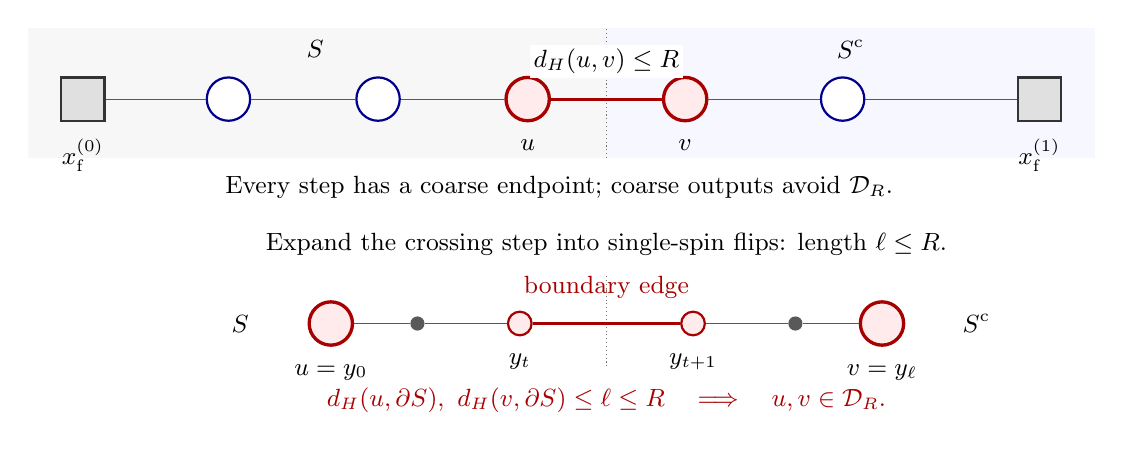
\begin{tikzpicture}[
  x=1cm,y=1cm,font=\small,
  coarse/.style={circle,draw=blue!55!black,fill=white,
    line width=.8pt,minimum size=5.5mm,inner sep=0pt},
  fine/.style={rectangle,draw=black!80,fill=black!12,
    line width=.8pt,minimum size=5.5mm,inner sep=0pt},
  forced/.style={coarse,draw=red!65!black,fill=red!8,line width=1.2pt},
  flip/.style={circle,fill=black!65,minimum size=1.8mm,inner sep=0pt},
  boundary/.style={circle,draw=red!65!black,fill=red!8,
    line width=.8pt,minimum size=3mm,inner sep=0pt}
]
  \fill[black!3] (-.05,-.75) rectangle (7.3,.9);
  \fill[blue!3] (7.3,-.75) rectangle (13.5,.9);
  \draw[densely dotted,black!55] (7.3,-.75) -- (7.3,.9);
  \node at (3.6,.63) {$S$};
  \node at (10.4,.63) {$S^{\mathrm c}$};

  \node[fine] (leftfine) at (.65,0) {};
  \node[coarse] (coarsezero) at (2.5,0) {};
  \node[coarse] (coarseone) at (4.4,0) {};
  \node[forced] (crossleft) at (6.3,0) {};
  \node[forced] (crossright) at (8.3,0) {};
  \node[coarse] (coarselast) at (10.3,0) {};
  \node[fine] (rightfine) at (12.8,0) {};
  \draw[black!65] (leftfine) -- (coarsezero)
    (coarsezero) -- (coarseone) (coarseone) -- (crossleft)
    (crossright) -- (coarselast) (coarselast) -- (rightfine);
  \draw[red!65!black,line width=1.1pt] (crossleft) -- (crossright);
  \node[below=1mm] at (leftfine.south) {$x_{\rm f}^{(0)}$};
  \node[below=1mm] at (rightfine.south) {$x_{\rm f}^{(1)}$};
  \node[below=1mm] at (crossleft.south) {$u$};
  \node[below=1mm] at (crossright.south) {$v$};
  \node[fill=white,inner sep=1.5pt] at (7.3,.48)
    {$d_H(u,v)\le R$};
  \node at (6.7,-1.12)
    {Every step has a coarse endpoint; coarse outputs avoid $\mathcal D_R$.};

  \node at (7.3,-1.85)
    {Expand the crossing step into single-spin flips: length $\ell\le R$.};
  \draw[densely dotted,black!55] (7.3,-2.25) -- (7.3,-3.4);
  \node[forced] (pathleft) at (3.8,-2.85) {};
  \node[flip] (pathone) at (4.9,-2.85) {};
  \node[boundary] (boundaryleft) at (6.2,-2.85) {};
  \node[boundary] (boundaryright) at (8.4,-2.85) {};
  \node[flip] (pathlast) at (9.7,-2.85) {};
  \node[forced] (pathright) at (10.8,-2.85) {};
  \draw[black!65] (pathleft) -- (pathone) (pathone) -- (boundaryleft)
    (boundaryright) -- (pathlast) (pathlast) -- (pathright);
  \draw[red!65!black,line width=1.1pt] (boundaryleft) -- (boundaryright);
  \node[above=2mm,red!65!black] at (7.3,-2.85) {boundary edge};
  \node[below=1mm] at (pathleft.south) {$u=y_0$};
  \node[below=1mm] at (boundaryleft.south) {$y_t$};
  \node[below=1mm] at (boundaryright.south) {$y_{t+1}$};
  \node[below=1mm] at (pathright.south) {$v=y_\ell$};
  \node at (2.65,-2.85) {$S$};
  \node at (12,-2.85) {$S^{\mathrm c}$};
  \node[red!65!black] at (7.3,-3.83)
    {$d_H(u,\partial S),\ d_H(v,\partial S)\le\ell\le R
      \quad\Longrightarrow\quad u,v\in\mathcal D_R$.};
\end{tikzpicture}
\caption{The boundary obstruction for the finite sequence of proposals.
In the upper chain, squares are fine endpoints and circles are coarse outputs; consecutive
configurations have Hamming distance at most $R$. When the fine endpoints lie on opposite sides, some consecutive pair
$u,v$ crosses the cut and contains a coarse output. A shortest path of
one-spin flips between that pair meets the two-sided boundary $\partial S$.
Its length is at most $R$, so both $u,v$ lie in
$\mathcal D_R=\{x:d_H(x,\partial S)\le R\}$, contradicting avoidance by
the coarse outputs. All geometry is schematic: grid outputs are
correlated, and lines do not represent continuous spin trajectories.}
\label{fig:connection}
\end{figure}


\paragraph{Avoiding a boundary selected from the target.}
At a fixed grid point, the driver difference $G-G(\theta)$ has
coordinate variance $2\delta$. Gaussian tails and a union bound over
spins show that the supremum of absolute energy differences is
$O(n\sqrt\delta)$, except with probability $O(e^{-cn})$.
On its complement, Gibbs weight ratios between the two disorders
are at most $\exp(O_\beta(n\sqrt\delta))$.

Apply the likelihood estimate \eqref{eq:6} with $l=b$. Its good
event depends only on this proposal run. If
$q_{\rm good}(dx\mid g)$ is the corresponding output
subprobability kernel, disintegration against the Gaussian disorder
marginal gives
\[
 q_{\rm good}(dx\mid g)
 \le\exp(n^{1-b/2})\pi_g(dx)
 \quad\text{for almost every }g.
\]
The primitive auxiliary inputs and final draw for this run are
independent of all matrix drivers. Thus, after fixing
$G(\theta)=g$ and adjoining $(G,G^\circ)$, this remains its
conditional good-output kernel. In particular, the inequality applies
to the random set $\mathcal D(G)$ once those matrices have been
fixed. The separate energy-change event is used to compare Gibbs
weights; it is not built into the proposal good event.

By \eqref{eq:12}, the resulting boundary probability on the
energy-change event's complement is at most
\[
 \exp\bigl(n^{1-b/2}+O_\beta(n\sqrt\delta)
                   -\tfrac12n^{1-b/20}\bigr).
\]
Add the proposal exceptional probability
$\exp(-n^{1-10b})$ and the energy-change exception. Since
$\sqrt\delta=n^{-f/8}$, this proves the required one-point
avoidance bound. Correlations with auxiliary inputs at other grid
points do not change this calculation.

\paragraph{Continuity of the coarse magnetizations.}
We next control the increments along the grid. At any grid point,
Proposition~\ref{prop:proposal} puts the Gram matrix of the coarse
$T_k$ within $n^{-b}$ of the identity except with probability
$\exp(-n^{1-10b})$. On this event all $|T_k|_n\le2$, and each
Gram--Schmidt residual has norm at least $1/2$. No fallback direction
is used. The reciprocals $1/s_k$ are bounded by a fixed power of $n$
on the deterministic coarse horizon, by \eqref{eq:1}.

For neighboring grid points satisfying these Gram conditions, we claim
\[
 |M_\theta(V_b)-M_{\theta'}(V_b)|_n
 \le(n^{C_1})^{K_b+1}|\theta-\theta'|,
 \qquad K_b=V_b/h,
 \tag{13}\label{eq:13}
\]
provided the primitive inputs have polynomially bounded norms.
The constant $C_1$ is independent of the grid and of $n$.

Here are the precise input bounds and the interval induction proving
this assertion. Bound the operator norms of
$W(G^\circ),W(G'_1),W(G'_2)$ and the normalized norms of all
completion vectors $z_k$ in the two input collections. For their
Brownian and bridge inputs, bound the supremum norms of cumulative
integrals against the deterministic coefficients $\rho$ and
$\sqrt{1-\rho^2}$. On a filled interval include only the centered
bridge in this primitive bound; its endpoint is handled separately.
All these norms are at most $n^3$ outside an event of probability
$O(e^{-cn})$. Gaussian tails give the matrix and vector estimates.
For the path integrals, write a bridge as Brownian motion minus
its linearly interpolated endpoint and use the Gaussian martingale
maximal bound for a bounded deterministic integrand. Rotation makes
the differences of the primitive inputs at two angles at most a
polynomial factor times $|\theta-\theta'|$.

At a Gram--Schmidt step, the difference of the two projection
operators is bounded by twice the sum of preceding direction
differences in $|\cdot|_n$. Normalizing residuals of norm at least
$1/2$ costs only a fixed factor. Using $1/s_k$, the new direction
difference is therefore controlled by earlier magnetization and
direction differences at polynomial cost. The same is true of the
new $g_k$, by its matrix-query and completion formula. The cumulative
driving signals from \eqref{eq:4} differ by the primitive integral
differences plus the endpoint difference multiplied by a deterministic
factor at most $\sqrt h$. Finally, the scalar integral equation
and its spatially Lipschitz drift control the differences in $Y$ and
$M$ over this interval at constant cost, by Gronwall's inequality.
Starting with the entirely auxiliary first interval and taking
successive maxima of these differences proves \eqref{eq:13} after
increasing $C_1$ if necessary.

Only the Gram conditions at the two endpoints of each grid step
were used. Since $K_b=O(n^{1/16}\log n)$ and the mesh spacing is
exponentially smaller, \eqref{eq:13} makes all consecutive coarse
magnetization differences negligible.

\paragraph{From magnetizations to spins.}
For either a coarse spin or a fine endpoint spin compared with its
own coarse magnetization, the normalized squared distance has mean
\[
 1-\mathbb E m_{V_b}^2=p(V_b)\le C_\beta n^{-b/2}.
\]
For a fine spin this follows from the martingale conditional mean
through the continuation. Under the unconditioned single-run law,
each squared distance is an average of bounded independent coordinate
variables. It is consequently at most $n^{-b/3}$ except with
probability $O(\exp(-n^{1-b}))$. The triangle inequality in
$|\cdot|_n$, together with the negligible magnetization increments,
then gives Hamming step sizes at most $R_n$ for large $n$.

We may now union bound all one-point and consecutive-point exceptions
for the two desired properties, including the primitive-input event.
The grid costs only $\exp(O(n^{1/4}))$, and $10b<d/2$.
The boundary exponent $1-b/20$ also exceeds $1-d/2$.
Thus the total failure probability is at most
$\exp(-n^{1-d/2})$ for sufficiently large $n$.

\paragraph{The crossing contradiction.}
On $\mathcal E$, Proposition~\ref{prop:coverage} gives each side of the
chosen cut fine-endpoint probability at least
$\exp(-n^{1-2d})$. Conditional independence therefore puts the
fine endpoints on opposite sides with probability at least
$\exp(-2n^{1-2d})$. But if both sequence properties hold, this
cannot happen. Some consecutive pair would cross the cut, and each
pair contains a coarse spin. A shortest one-spin path between that
pair meets $\partial S$ and has length at most $R_n$, placing
that coarse spin in $\mathcal D(G)$.

Consequently
\[
 \Pr(\mathcal E)\exp(-2n^{1-2d})
 \le\exp(-n^{1-d/2}).
\]
Since $d/2<2d$, this implies $\Pr(\mathcal E)=o(1)$ and proves
\eqref{eq:11}. The auxiliary diagonal and smoothing base are used
only in this proof; the resulting flow bound concerns the original
heat bath.
\end{proof}

\FloatBarrier
\setcounter{equation}{13}
\section{From balanced flows to typical-state mixing}\label{sec:mixing}

The flow estimate is available only when both sides of a cut have
appreciable Gibbs mass. The following finite-state argument is adapted
to exactly that information. It first finds a large set with internal
expansion, then uses the full chain's entropy dissipation to control
typical starting states. There is no requirement that a trajectory
remain in the large set.

\begin{lemma}[Pruning and averaged mixing]\label{lem:pruning}
Let $\Omega$ be a finite set, let $\pi$ be a strictly positive
probability on $\Omega$, and let $P_t$ be a continuous-time Markov
semigroup reversible with respect to $\pi$, with jump rates $c(x,y)$.
Assume that, for some $R>0$,
\[
 \sum_{y\ne x}c(x,y)\le R\qquad(x\in\Omega).
\]
Let $0<\varepsilon<1/3$ and $B>0$. Suppose
\[
 Q(S,S^{\rm c}):=\sum_{x\in S,\,y\notin S}\pi(x)c(x,y)>B
 \quad\text{whenever }\varepsilon\le\pi(S)\le1-\varepsilon.
\]
Then for every $T>0$,
\begin{equation}\label{eq:averaged-mixing}
 \sum_{x\in\Omega}\pi(x)\|P_T(x,\cdot)-\pi\|_{\rm TV}
 \le\frac{\sqrt{2R H(\pi)}}{B\sqrt T}+2\varepsilon,
 \qquad H(\pi)=-\sum_x\pi(x)\log\pi(x).
\end{equation}
\end{lemma}

\begin{proof}
Put $q(x,y)=\pi(x)c(x,y)=q(y,x)$, and use the unordered-edge
Dirichlet form
\[
 \mathfrak D(u)=\sum_{\{x,y\}}q(x,y)(u(x)-u(y))^2.
\]
Only distinct vertices occur, and every unordered pair is counted once.

\paragraph{Removing sets that do not expand.}
Start with $C=\Omega$. Whenever a nonempty $U\subset C$ satisfies
\[
 \pi(U)\le\pi(C)/2,\qquad Q(U,C\setminus U)<B\pi(U),
\]
remove $U$ from $C$. This process terminates because each removal
eliminates a vertex. If $A$ denotes all vertices removed so far,
then every edge between $A$ and its current complement was counted
when its first endpoint was removed. Thus, whenever $A\ne\varnothing$,
\[
 Q(A,\Omega\setminus A)<B\pi(A).
\]
Suppose the removed mass first reached $\varepsilon$. Its preceding
mass $a$ was less than $\varepsilon$, and the newly removed set has
mass at most $(1-a)/2$. The new total is therefore at most
$(1+a)/2<(1+\varepsilon)/2<1-\varepsilon$. This contradicts
the balanced-cut hypothesis, since $B\pi(A)\le B$.
Consequently the terminal set satisfies $\pi(C)>1-\varepsilon$
and
\begin{equation}\label{eq:internal-expansion}
 Q(U,C\setminus U)\ge B\pi(U)
 \quad\text{for every }U\subset C\text{ with }\pi(U)\le\pi(C)/2.
\end{equation}

\paragraph{A Poincar\'e inequality on the retained set.}
We use the coarea proof of the reversible Cheeger inequality
\cite[Theorem~3.5]{LawlerSokal1988}, keeping the original,
unnormalized weights on $C$. The resulting estimate is
\begin{equation}\label{eq:14}
 \sum_{y\in C}\pi(y)(u(y)-\bar u_C)^2
 \le\frac{2R}{B^2}\mathfrak D(u),
 \qquad \bar u_C=\frac1{\pi(C)}\sum_{y\in C}\pi(y)u(y).
\end{equation}
To prove it, choose a weighted median $m$ of $u$ on $C$. Each of
$w=(u-m)_+$ and $w=(m-u)_+$ has support of mass at most
$\pi(C)/2$. Integrating \eqref{eq:internal-expansion} over the
level sets of $w^2$ gives
\[
 B\sum_C\pi w^2
 \le\sum_{\{x,y\}\subset C}q(x,y)|w(x)^2-w(y)^2|.
\]
By Cauchy--Schwarz this is at most
\[
 \left(\sum_{\{x,y\}\subset C}q(x,y)(w(x)-w(y))^2\right)^{1/2}
 \left(2R\sum_C\pi w^2\right)^{1/2}.
\]
Indeed, $(w(x)+w(y))^2\le2(w(x)^2+w(y)^2)$, and the total outgoing
rate is at most $R$. If $\sum_C\pi w^2$ vanishes, its estimate
is immediate; otherwise divide and square. The sum of the energies
of the positive and negative parts is at most $\mathfrak D(u)$.
The weighted mean minimizes squared error, proving \eqref{eq:14}.

\paragraph{Entropy dissipation for the full chain.}
For a fixed starting state $x$, set $f_t^x(y)=P_t(x,y)/\pi(y)$.
Reversibility and
\[
 (a-b)(\log a-\log b)\ge4(\sqrt a-\sqrt b)^2
 \qquad(a,b>0)
\]
yield the entropy-dissipation estimate
\cite[Lemmas~2.5 and~2.7]{DiaconisSaloffCoste1996}
\begin{equation}\label{eq:15}
 \int_0^T\sum_x\pi(x)\mathfrak D(\sqrt{f_t^x})\,dt
 \le\frac14H(\pi).
\end{equation}
Indeed, the derivative of $\sum_y\pi(y)f_t^x(y)\log f_t^x(y)$ is
\[
 -\sum_{\{y,z\}}q(y,z)
       (f_t^x(y)-f_t^x(z))(\log f_t^x(y)-\log f_t^x(z)).
\]
The initial entropy is $\log(1/\pi(x))$, and the final entropy is
nonnegative. Averaging in $x\sim\pi$ and integrating proves
\eqref{eq:15}. Vanishing densities and reducible chains cause no
problem: start instead with $(1-\eta)f_0^x+\eta$ and pass to
$\eta\downarrow0$, or calculate on communicating classes.

\paragraph{Averaging fixed-state distances.}
Combining \eqref{eq:14} and \eqref{eq:15} supplies some
$t\in(0,T]$ for which
\[
 \sum_x\pi(x)r_x^2\le\frac{R H(\pi)}{2TB^2},
 \qquad r_x^2=\sum_C\pi(y)(\sqrt{f_t^x(y)}-a_x)^2,
 \qquad a_x=\frac1{\pi(C)}\sum_C\pi(y)\sqrt{f_t^x(y)}.
\]
Cauchy--Schwarz and
$a_x^2\pi(C)\le\sum_C\pi f_t^x\le1$ imply
\[
 \sum_C\pi|f_t^x-a_x^2|\le2r_x.
\]
Also, total normalization gives
$|\sum_C\pi(f_t^x-1)|\le\sum_{C^{\rm c}}\pi(f_t^x+1)$.
Comparing $f_t^x$ first with $a_x^2$ and then with $1$ on $C$,
and adding the complement, yields
\[
 \sum_\Omega\pi|f_t^x-1|
 \le4r_x+2\sum_{C^{\rm c}}\pi(f_t^x+1).
\]
The last sum before its factor two has average $2\pi(C^{\rm c})$
over $x\sim\pi$, because stationarity gives
$\sum_x\pi(x)f_t^x(y)=1$. Dividing by two for total variation
and applying Cauchy--Schwarz in $x$ proves the desired upper bound
at this time $t$. Contraction under $P_{T-t}$ gives the same bound
at the prescribed time $T$, establishing \eqref{eq:averaged-mixing}.
\end{proof}

\begin{proof}[Proof of Theorem~\ref{thm:main}]
On the disorder event of Proposition~\ref{prop:cuts}, apply
Lemma~\ref{lem:pruning} with
\[
 \varepsilon=n^{-d},\qquad B=\exp(-n^{1-b/20}),\qquad R=n.
\]
The last choice is valid because there are $n$ rate-one update
clocks. Also $H(\pi_G)\le n\log2$, since the state space has
$2^n$ elements. Hence
\[
 \sum_x\pi_G(x)\|P_T^G(x,\cdot)-\pi_G\|_{\rm TV}
 \le\frac{\sqrt{2\log2}\,n}{B\sqrt T}+2n^{-d}.
\]
Take $T=\exp(n^{1-b/40})$. The first term tends to zero, as
\[
 \log\frac{n}{B\sqrt T}
 =\log n+n^{1-b/20}-\tfrac12n^{1-b/40}\longrightarrow-\infty.
\]
The flow event itself has disorder probability tending to one.
Markov's inequality therefore shows that the Gibbs mass of fixed
states whose distance at time $T$ exceeds $1/4$ tends to zero in
disorder probability. The added diagonal changes neither this Gibbs
law nor the transition rates, so the same statement holds for the
model in \eqref{eq:intro-model}. This proves the theorem with
\[
 c_\beta=b/40=1/40000000.
\]
All threshold dimensions may depend on the fixed $\beta>1$.
\end{proof}

\begin{thebibliography}{99}

\bibitem{AC2015}
A.~Auffinger and W.-K.~Chen,
\newblock On properties of Parisi measures,
\newblock \emph{Probability Theory and Related Fields}
\textbf{161} (2015), 817--850.
\newblock \href{https://doi.org/10.1007/s00440-014-0563-y}{doi:10.1007/s00440-014-0563-y};
\href{https://arxiv.org/abs/1303.3573v1}{arXiv:1303.3573v1}.

\bibitem{BLO2026}
M.~Boban, A.~Li and S.~Oveis Gharan,
\newblock Rank-1-perturbed trickledown theorems: mixing time of Glauber
dynamics for the Sherrington--Kirkpatrick model up to
$\beta\leq\frac12+\varepsilon$,
\newblock preprint (2026),
\href{https://arxiv.org/abs/2609.13138v1}{arXiv:2609.13138v1}.

\bibitem{BKM2005}
V.~I. Bogachev, A.~V. Kolesnikov and K.~V. Medvedev,
\newblock Triangular transformations of measures,
\newblock \emph{Sbornik: Mathematics} \textbf{196} (2005), no.~3, 309--335.
\newblock \href{https://doi.org/10.1070/SM2005v196n03ABEH000882}{doi:10.1070/SM2005v196n03ABEH000882}.

\bibitem{Bolthausen2014}
E.~Bolthausen,
\newblock An iterative construction of solutions of the TAP equations
for the Sherrington--Kirkpatrick model,
\newblock \emph{Communications in Mathematical Physics}
\textbf{325} (2014), 333--366.
\newblock \href{https://doi.org/10.1007/s00220-013-1862-3}{doi:10.1007/s00220-013-1862-3};
\href{https://arxiv.org/abs/1201.2891}{arXiv:1201.2891}.

\bibitem{BLM2013}
S.~Boucheron, G.~Lugosi, and P.~Massart,
\newblock \emph{Concentration Inequalities: A Nonasymptotic Theory of Independence},
\newblock Oxford University Press, 2013.
\newblock \href{https://doi.org/10.1093/acprof:oso/9780199535255.001.0001}{Publisher reference}.

\bibitem{Chen2017}
W.-K.~Chen,
\newblock Variational representations for the Parisi functional and
the two-dimensional Guerra--Talagrand bound,
\newblock \emph{Annals of Probability} \textbf{45} (2017),
no.~6A, 3929--3966.
\newblock \href{https://doi.org/10.1214/16-AOP1154}{doi:10.1214/16-AOP1154};
\href{https://arxiv.org/abs/1501.06635v2}{arXiv:1501.06635v2}.

\bibitem{DiaconisSaloffCoste1996}
P.~Diaconis and L.~Saloff-Coste,
\newblock Logarithmic Sobolev inequalities for finite Markov chains,
\newblock \emph{Annals of Applied Probability} \textbf{6} (1996),
no.~3, 695--750.
\newblock \href{https://doi.org/10.1214/aoap/1034968224}{doi:10.1214/aoap/1034968224}.

\bibitem{EKZ2022}
R.~Eldan, F.~Koehler and O.~Zeitouni,
\newblock A spectral condition for spectral gap: fast mixing in
high-temperature Ising models,
\newblock \emph{Probability Theory and Related Fields}
\textbf{182} (2022), nos.~3--4, 1035--1051.
\newblock \href{https://doi.org/10.1007/s00440-021-01085-x}{doi:10.1007/s00440-021-01085-x};
\href{https://arxiv.org/abs/2007.08200v1}{arXiv:2007.08200v1}.
The section cited here refers to this preprint version.

\bibitem{Guerra2003}
F.~Guerra,
\newblock Broken replica symmetry bounds in the mean field spin glass model,
\newblock \emph{Communications in Mathematical Physics}
\textbf{233} (2003), 1--12.
\newblock \href{https://doi.org/10.1007/s00220-002-0773-5}{doi:10.1007/s00220-002-0773-5};
\href{https://arxiv.org/abs/cond-mat/0205123v1}{arXiv:cond-mat/0205123v1}.

\bibitem{JT2017}
A.~Jagannath and I.~Tobasco,
\newblock Some properties of the phase diagram for mixed $p$-spin glasses,
\newblock \emph{Probability Theory and Related Fields}
\textbf{167} (2017), 615--672.
\newblock \href{https://doi.org/10.1007/s00440-015-0691-z}{doi:10.1007/s00440-015-0691-z};
\href{https://arxiv.org/abs/1504.02731v2}{arXiv:1504.02731v2}.
Numbered propositions and corollaries cited here refer to this preprint version.

\bibitem{LawlerSokal1988}
G.~F. Lawler and A.~D. Sokal,
\newblock Bounds on the $L^2$ spectrum for Markov chains and Markov
processes: a generalization of Cheeger's inequality,
\newblock \emph{Transactions of the American Mathematical Society}
\textbf{309} (1988), no.~2, 557--580.
\newblock \href{https://doi.org/10.1090/S0002-9947-1988-0930082-9}{doi:10.1090/S0002-9947-1988-0930082-9}.

\bibitem{Lopatto2026}
P.~Lopatto,
\newblock Full replica symmetry breaking in the Sherrington--Kirkpatrick model,
\newblock preprint (2026),
\href{https://arxiv.org/abs/2607.11756v3}{arXiv:2607.11756v3}.

\bibitem{LugosiNeu2022}
G.~Lugosi and G.~Neu,
\newblock Generalization bounds via convex analysis,
\newblock \emph{Proceedings of Machine Learning Research}
\textbf{178} (2022), 3524--3546.
\newblock \href{https://proceedings.mlr.press/v178/lugosi22a.html}{Proceedings article}.

\bibitem{Montanari2021}
A.~Montanari,
\newblock Optimization of the Sherrington--Kirkpatrick Hamiltonian,
\newblock \emph{SIAM Journal on Computing}
\textbf{54} (2025), no.~4, FOCS19-1--FOCS19-38
(first published online 2021).
\newblock \href{https://doi.org/10.1137/20M132016X}{doi:10.1137/20M132016X};
\href{https://arxiv.org/abs/1812.10897v2}{arXiv:1812.10897v2}.
Numbered sections cited here refer to this preprint version.

\bibitem{OpenAISKBarriers2026}
OpenAI,
\newblock Stretched-exponential barriers for typical SK initial states,
\newblock OpenAI Math Release preprint
\href{https://github.com/openai/math/blob/main/preprints/Stretched-exponential-barriers-for-typical-SK-initial-states-September-24-2026/paper.pdf}{OAI:Stretched-exponential-barriers-for-typical-SK-initial-states-September-24-2026},
2026.

\bibitem{Sellke2025}
M.~Sellke,
\newblock Exponentially slow mixing of the low temperature SK model,
\newblock preprint (2025),
\href{https://arxiv.org/abs/2511.22621v2}{arXiv:2511.22621v2}.

\bibitem{SK1975}
D.~Sherrington and S.~Kirkpatrick,
\newblock Solvable model of a spin-glass,
\newblock \emph{Physical Review Letters}
\textbf{35} (1975), no.~26, 1792--1796.
\newblock \href{https://doi.org/10.1103/PhysRevLett.35.1792}{doi:10.1103/PhysRevLett.35.1792}.

\bibitem{Wang2026}
S.~Wang,
\newblock Optimal mixing of Glauber dynamics for the
Sherrington--Kirkpatrick model at $\beta<1/2$,
\newblock preprint (2026),
\href{https://arxiv.org/abs/2608.22159v2}{arXiv:2608.22159v2}.

\bibitem{Zhou2026}
Y.~Zhou,
\newblock Existence of full replica symmetry breaking for the
Sherrington--Kirkpatrick model at low temperature,
\newblock \emph{Communications on Pure and Applied Mathematics}
\textbf{79} (2026), 1746--1770.
\newblock \href{https://doi.org/10.1002/cpa.70038}{doi:10.1002/cpa.70038}.

\end{thebibliography}

\end{document}
